\section{Experiments}
\label{sec:setup}

Our experiments evaluate whether a single model can improve its own
next-tool-call speculation while preserving downstream task performance. We
first describe the evaluation setup, then report main results across search and
conversational tool-use benchmarks, analyze cross-domain generalization, and
ablate the stabilization techniques used in joint agent-speculator RL.

\subsection{Experimental Setup}
\label{sec:experiments:setup}

\paragraph{Tasks and environments.}
We evaluate on two families of structured tool-use tasks. Agentic
SearchQA~\citep{jin2025searchr1,song2025r1searcher} requires the model to
answer multi-hop questions by issuing search calls and reasoning over returned
evidence. $\tau$-bench conversational tool-use
tasks~\citep{yao2024taubench,barres2025tau2bench} require the agent to interact
with a simulated user and complete airline or retail tasks through
schema-constrained APIs. These settings stress complementary aspects of
speculation: SearchQA emphasizes query formulation under partial information,
whereas $\tau$-bench emphasizes exact API selection and argument filling in
long-horizon interactions.

\paragraph{Training and evaluation data.}
For Agentic SearchQA settings, we train on FlashQA and evaluate on HotpotQA,
MuSiQue, and BrowseComp-Plus (BCP)~\citep{chen2025browsecompplus}.
For BCP, we follow~\citet{sun2025contextfolding} and use the 150-query evaluation split from their
680/150 train--test partition. We also follow the official BCP setup 
to use Qwen3-Embed-0.6B as the dense retriever. For
conversational tool-use tasks, we train on
ToolScale~\citep{su2025toolorchestra} and evaluate on $\tau$-bench Airline and
$\tau$-bench Retail~\citep{barres2025tau2bench}.

\paragraph{Models and baselines.}
We instantiate our method with Qwen3-4B~\citep{yang2025qwen3} and
Qwen3.5-4B~\citep{qwen2026qwen35modelcard}. We compare against smaller same-family
LLMs as the external speculators, the base 4B agent prompted to predict its own next call,
and the SFT-warmup checkpoint before RL. Specifically, the external speculators are
Qwen3-0.6B and Qwen3-1.7B for Qwen3-4B, and Qwen3.5-0.8B and Qwen3.5-2B for
Qwen3.5-4B. We employ same speculation suffix for all models. 

\paragraph{Training protocol.}
We follow the joint agent-speculator RL recipe in
Section~\ref{sec:method:training-recipe}. Each run begins with a short SFT
warmup on a mix of successful trajectories and speculation examples so that the model can emit well-formed tool
calls under the speculation suffix before RL begins. We then instanstite the alternative RL between
agent updates and speculator updates, resetting optimizer state when the
schedule switches modes. Unless otherwise noted, we use DAPO-style grouped
policy optimization~\citep{yu2025dapo} with $G_{\mathrm{ag}}=8$ agent rollouts,
$G_{\mathrm{sp}}=8$ speculator rollouts, learning rate $3\times10^{-6}$, and a
fixed 200-step budget per RL training. Appendix~\ref{sec:appendix:training-hyperparameters}
lists the remaining implementation details, such as the training hardware.

% All ablations use the same data split, rollout budget, and base model as the corresponding full run.

\paragraph{Evaluation protocol and metrics.}
For speculation evaluation, we first run the model in agent mode and collect
complete trajectories. At each tool-call turn, we truncate the trajectory
immediately before the call, append the speculation suffix, and ask the
speculator to predict the next call. We report Hit@1 exact match, where a hit
requires both the tool name and the full argument dictionary to match the
agent's eventual call. For task quality, we report task success on HotpotQA,
MuSiQue, BCP, $\tau$-bench Airline, and $\tau$-bench Retail. For external
speculators, task success refers to the fixed target 4B agent whose calls are
being predicted, not to the smaller draft model as an independent agent.
Together, these metrics capture the central trade-off: speculation is useful
only if it improves reusable call prediction without degrading task behavior.

\subsection{Main Results}
\label{sec:results}

Table~\ref{tab:main-self-speculation} reports the main results across both model
families and evaluation domains. We highlight the following observations:

\paragraph{Joint agent-speculator RL improves speculation performance.}
Table~\ref{tab:main-self-speculation} extends the finding from
Section~\ref{sec:empirical-self-speculate}: the deployed agent is already a
stronger speculator for itself than smaller same-family draft models. In the
Qwen3 series, the strongest external speculator averages 18.6 Hit@1, while the
base 4B agent reaches 29.1 when prompted to predict its own next call. 
We also highlight that the SFT warmup improves this self-speculation ability, raising average Hit@1 to
44.1 for Qwen3-4B and 48.9 for Qwen3.5-4B. The joint agent-speculator RL method further
improves average Hit@1 to 61.2 and 66.3, respectively, with gains in the same direction on every benchmark. 
Since Hit@1 requires both the tool name and full argument dictionary to match, 
these gains indicate better speculation timing gains.

\paragraph{Agent performance is largely preserved.}
Since the same parameter set is used in both agent and speculator modes for our self-sepculative agent, improving
next-call prediction can risk degrading task solving performance. In
Table~\ref{tab:main-self-speculation}, we observe that task success remains stable after RL,
average success changes from 26.6 to 27.7 for Qwen3-4B and from 49.2 to 50.6
for Qwen3.5-4B. These results confirm the same pattern, with no
systematic degradation across search QA or conversational tool-use benchmarks.
Thus, the speculation gains above are not obtained by sacrificing the deployed
agent's end-task performance; our joint agent-speculator RL achieves accurate
speculation while keeping the agent policy usable.

\subsection{Generalization Across Domains}
\label{sec:analysis:generalization}

An interesting question to ask is whether the ability to self-speculate
generalizes across domains. We investigate this by evaluating checkpoints
trained on one agent task in the other: the SearchQA-trained Qwen3-4B checkpoint
is tested on $\tau$-bench, and the ToolScale-trained Qwen3.5-4B checkpoint is
tested on SearchQA. Table~\ref{tab:domain-generalization} shows that next-call
prediction transfers across domains, while end-task success is less stable. For
example, the SearchQA-trained Qwen3-4B checkpoint improves Airline/Retail Hit@1
from 35.6/39.7 to 45.6/50.1 after RL, while task success drops from 21.6/36.4
to 17.6/29.8. In the reverse direction, the ToolScale-trained Qwen3.5-4B
checkpoint improves HotpotQA/MuSiQue Hit@1 from 25.4/28.3 to 35.4/37.9 after
RL, while task success also decreases. This suggests that the training procedure
teaches transferable call-level behavior, such as matching common tool-call
arguments, but successful task completion still depends on domain-specific
reasoning and interaction strategy. Matched-domain agentic RL training is
therefore important for preserving task success in the target domain.

\begin{table}[t]
\centering
\renewcommand{\arraystretch}{1.08}
\small
\setlength{\tabcolsep}{1.2pt}
\resizebox{0.95\columnwidth}{!}{%
\begin{tabular}{@{}l|cc|cc|cc|cc@{}}
\toprule \midrule
\multirow{2}{*}{Model} &
\multicolumn{2}{c|}{\textbf{HotpotQA}} &
\multicolumn{2}{c|}{\textbf{MuSiQue}} &
\multicolumn{2}{c|}{\textbf{Tau-Air}} &
\multicolumn{2}{c}{\textbf{Tau-Ret}} \\
\cmidrule(lr){2-3} \cmidrule(lr){4-5} \cmidrule(lr){6-7} \cmidrule(lr){8-9}
 & H@1 & Succ. & H@1 & Succ. & H@1 & Succ. & H@1 & Succ. \\
\midrule
\rowcolor{transgray}
\multicolumn{9}{c}{\textbf{Qwen3-4B}} \\
\midrule
Base & 23.2 & \textbf{52.1} & 26.4 & \textbf{15.1} & 35.6 & \textbf{21.6} & 39.7 & \textbf{36.4} \\
SFT & 37.8 & 49.4 & 40.9 & 13.8 & 41.2 & 18.9 & 45.8 & 32.0 \\
RL & \textbf{55.2} & 48.6 & \textbf{58.4} & 12.9 & \textbf{45.6} & 17.6 & \textbf{50.1} & 29.8 \\
\midrule
\rowcolor{transgray}
\multicolumn{9}{c}{\textbf{Qwen3.5-4B}} \\
\midrule
Base & 25.4 & \textbf{63.1} & 28.3 & \textbf{25.1} & 42.1 & \textbf{56.4} & 46.8 & \textbf{69.7} \\
SFT & 31.8 & 60.0 & 34.2 & 22.8 & 58.6 & 53.1 & 62.9 & 66.0 \\
RL & \textbf{35.4} & 57.9 & \textbf{37.9} & 21.6 & \textbf{76.1} & 51.4 & \textbf{79.4} & 63.7 \\
\midrule
\bottomrule
\end{tabular}
}
\caption{Generalization across domains. We evaluate whether a self-speculator
trained in one interaction family transfers to the other.}
\label{tab:domain-generalization}
\vspace{-0.12in}
\end{table}


\subsection{Ablation Study}
\label{sec:ablation}

We ablate the stabilization techniques in the joint training recipe on SearchQA
with Qwen3-4B.
Figure~\ref{fig:reward-ablation-trends} shows training-time reward traces when
removing SFT warmup, optimizer reset, or alternating schedule, while
Table~\ref{tab:alternating-schedule} compares different agent:speculator update
schedules under the same iteration budget.

\paragraph{Effect of SFT warmup.}
The w/o SFT warmup variant starts RL directly from the base model, testing
whether the speculation suffix alone is enough to induce well-formed
call-prediction behavior. In Figure~\ref{fig:reward-ablation-trends}, this
variant lags the full method in speculation reward and is less stable early in
training. This suggests that warmup provides a useful initialization before RL
optimizes next-call prediction accuracy, because early updates can otherwise
spend capacity on discovering the output format rather than matching the
agent's eventual call.

\begin{figure}[t]
\centering
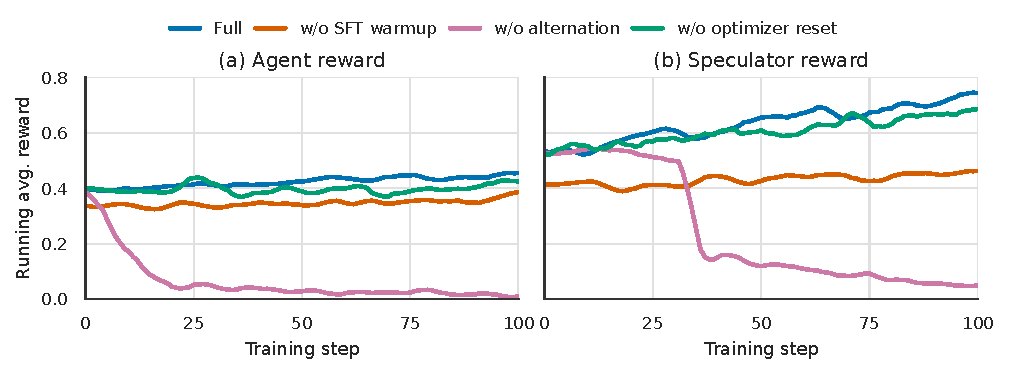
\includegraphics[width=0.98\linewidth]{figures/reward_ablation_trends.pdf}
\caption{Reward trend over the first 100 steps for each mode:
(left) agent reward and (right) speculator reward. The full method
preserves agent reward while improving speculator reward. Removing SFT warmup,
optimizer resets, or alternating updates leads to weaker or less stable reward trends.}
\label{fig:reward-ablation-trends}
\vspace{-0.14in}
\end{figure}

\paragraph{Effect of optimizer reset.}
The w/o optimizer reset variant keeps the alternating schedule but preserves
optimizer state across mode switches. In
Figure~\ref{fig:reward-ablation-trends}, it produces weaker and less stable
reward trends than the full method. The two modes optimize different targets:
agent updates improve task-solving behavior, while speculator updates improve
next-call prediction. If the same optimizer state is carried from one mode into
the other, momentum and adaptive statistics from the previous target can push the
new updates in a less useful direction~\citep{sutskever2013momentum,kingma2015adam}.
Resetting the optimizer at each mode switch gives each block a fresh optimizer
state and makes training more stable by limiting cross-mode interference through
optimizer history.

\paragraph{Effect of alternating updates.}
The w/o alternating updates trace in Figure~\ref{fig:reward-ablation-trends}
shows that mixing agent and speculator updates leads to early collapse in training. Table~\ref{tab:alternating-schedule} compares block schedules under
the same iteration budget. Switching every step is worst: the 1:1 schedule
achieves only 31.8 average Hit@1 and 10.3 average task success. Performance
improves as each mode is trained for longer consecutive updates, reaching 55.2
average Hit@1 and 26.1 average task success with the 4:8 schedule. This suggests
that the speculator needs enough consecutive signal to track the agent's current
call distribution, while the agent still needs periodic updates to preserve task
performance.

\begin{table}[t]
\centering
\scriptsize
\setlength{\tabcolsep}{1.4pt}
\resizebox{0.95\columnwidth}{!}{%
\begin{tabular}{@{}r|cc|cc|cc|cc@{}}
\toprule \midrule
\multirow{2}{*}{\begin{tabular}{@{}c@{}}$m(k)$\\schedule\end{tabular}} &
\multicolumn{2}{c|}{\textbf{Hotpot}} &
\multicolumn{2}{c|}{\textbf{MuSiQ}} &
\multicolumn{2}{c|}{\textbf{BCP}} &
\multicolumn{2}{c}{\textbf{Avg.}} \\
\cmidrule(lr){2-3} \cmidrule(lr){4-5} \cmidrule(lr){6-7} \cmidrule(lr){8-9}
 & H@1$\uparrow$ & Succ.$\uparrow$
 & H@1$\uparrow$ & Succ.$\uparrow$
 & H@1$\uparrow$ & Succ.$\uparrow$
 & H@1$\uparrow$ & Succ.$\uparrow$ \\
\midrule
1:1 & 31.8 & 18.4 & 34.6 & 6.8 & 29.1 & 5.6 & 31.8 & 10.3 \\
2:2 & 41.9 & 39.6 & 44.7 & 13.9 & 38.8 & 15.2 & 41.8 & 22.9 \\
4:4 & 50.1 & 49.8 & 53.2 & 16.3 & 47.5 & 7.2 & 50.3 & 24.4 \\
4:8 & \textbf{55.2} & \textbf{53.0} & \textbf{58.4} & \textbf{17.1} & \textbf{52.1} & \textbf{8.1} & \textbf{55.2} & \textbf{26.1} \\
\midrule
\bottomrule
\end{tabular}
}
\caption{Ablation over agent:speculator update schedules on SearchQA. We report
Hit@1 and task success on the three search datasets used in the main table.}
\label{tab:alternating-schedule}
\vspace{-0.12in}
\end{table}

